\documentclass[11pt]{article}
% =========================================================================
% SHARED STYLE FILE for 11_Master_Projects reports
% Visual style follows 0_Thesis_Submission/24m0553_AK_Gaurav_Mtech_Report.pdf:
% serif body font, blue hyperlinked TOC/links, ruled section headings,
% IITB-style title page, formal academic report structure.
% =========================================================================

\usepackage[a4paper,margin=1in]{geometry}
\usepackage{xcolor}
\usepackage{graphicx}
\graphicspath{{../images/}}
\usepackage{amsmath,amssymb}
\usepackage{booktabs}
\usepackage{caption}
\usepackage{float}
\usepackage[hidelinks]{hyperref}
\usepackage{titlesec}
\usepackage{enumitem}
\usepackage{setspace}
\usepackage[T1]{fontenc}
\usepackage{lmodern}
\usepackage{microtype}

% Every \includegraphics call is automatically framed with a thin black
% border (matches the printed look of figures/photos/charts in the source
% reports). \oldincludegraphics is kept available for institutional
% logos/seals on title pages, which should remain unframed.
\let\oldincludegraphics\includegraphics
\setlength{\fboxsep}{1pt}
\setlength{\fboxrule}{0.6pt}
\renewcommand{\includegraphics}[2][]{\fbox{\oldincludegraphics[#1]{#2}}}

\definecolor{thesisblue}{RGB}{0,0,205}
\hypersetup{
  colorlinks=true,
  linkcolor=thesisblue,
  urlcolor=thesisblue,
  citecolor=thesisblue,
  filecolor=thesisblue
}

\onehalfspacing
\setlength{\parskip}{6pt}
\setlength{\parindent}{0pt}

\titleformat{\section}
  {\normalfont\Large\bfseries}{\thesection}{1em}{}
\titleformat{\subsection}
  {\normalfont\large\bfseries}{\thesubsection}{1em}{}
\titleformat{\subsubsection}
  {\normalfont\normalsize\bfseries}{\thesubsubsection}{1em}{}

\newcommand{\reportTitlePage}[7]{%
  % #1 = Report title
  % #2 = Course code & name (e.g. "CE 605: Applied Statistics")
  % #3 = Subtitle/topic line (e.g. "Project Report 2: Network Analysis")
  % #4 = Author block (can be multi-line with \\ for group projects)
  % #5 = Supervisor name(s)
  % #6 = Programme line (e.g. "M.Tech in Transportation Systems Engineering")
  % #7 = Month/Year
  \begin{titlepage}
    \centering
    \vspace*{0.5cm}
    {\large\bfseries #2}\par
    \vspace{0.3cm}
    {\Large\bfseries #3}\par
    \vspace{1.2cm}
    {\Huge\bfseries #1}\par
    \vspace{1.5cm}
    \oldincludegraphics[width=3.2cm]{../../assets/iitb_logo.png}\par
    \vspace{1.2cm}
    Submitted by:\par
    \vspace{0.2cm}
    {\bfseries #4}\par
    \vspace{0.8cm}
    Under the Supervision of\par
    \vspace{0.2cm}
    {\bfseries #5}\par
    \vspace{1.2cm}
    #6\par
    Department of Civil Engineering\par
    \textbf{Indian Institute of Technology Bombay}\par
    Mumbai -- 400076, India\par
    \vspace{0.3cm}
    #7\par
  \end{titlepage}
}

\newcommand{\reportAbstract}[1]{%
  \section*{Abstract}
  #1
  \vspace{0.5cm}
}


\title{Urban Transport Accessibility in India: A Comparative Study of PTAL Scores in Bangalore and Varanasi}
\author{Abhijeet Kumar Gaurav}
\date{}

\begin{document}

\begin{titlepage}
  \centering
  \vspace*{0.3cm}
  {\large\bfseries UG Project Report submitted in partial fulfilment for the award of the degree of}\par
  \vspace{0.2cm}
  {\large\bfseries Bachelor of Technology}\par
  \vspace{1cm}
  {\Huge\bfseries ``Urban Transport Accessibility in India: A Comparative Study of PTAL Scores in Bangalore and Varanasi''}\par
  \vspace{1.5cm}
  By\par
  \vspace{0.2cm}
  {\bfseries Abhijeet Kumar Gaurav \\ (20065001)}\par
  \vspace{0.8cm}
  Under the Guidance of\par
  \vspace{0.2cm}
  {\bfseries Dr.\ Abhisek Mudgal} \\ Assistant Professor\par
  \vspace{1.2cm}
  \oldincludegraphics[width=2.6cm]{fig_iitbhu_logo.png}\par
  \vspace{1cm}
  Department of Civil Engineering\par
  \textbf{Indian Institute of Technology (Banaras Hindu University)}\par
  Varanasi -- 221005\par
  \vspace{0.3cm}
  Jan--Nov 2023\par
\end{titlepage}

\pagenumbering{roman}

\reportAbstract{
Public transport ensures a city's economic and social well-being by facilitating efficient
mobility, reducing automobile dependence, and mitigating traffic congestion, and one of the key
determinants of a well-functioning public transport system is the level of accessibility it
offers. This project evaluates the Public Transport Accessibility Level (PTAL) in Bangalore,
emphasising the Bangalore Metropolitan Transport Corporation (BMTC) mode, and extends the
analysis to Varanasi's public bus network. Drawing on the PTAL methodology originated by
London's Borough of Hammersmith and Fulham and subsequently adopted by Transport for London
(TfL), the model is adapted to India's urban context using a grid-based variant: the study area
is segmented into 1~km\textsuperscript{2} grid cells, whose centroids serve as points of
interest (POIs), and PTAL is computed with respect to bus stops as service access points (SAPs).
A Geographic Information System (GIS) mapping workflow (QGIS with Python scripting) is used to
represent PTAL levels visually, considering average walk speed and time, distances to public
transport stops, and average frequencies of public transport modes. In addition to PTAL mapping,
a comparative regression analysis of PTAL score against population was conducted for both
cities. The findings show that while both Bangalore and Varanasi have experienced population
growth, the relationship between population and PTAL score differs: Varanasi exhibits a weak,
statistically significant \emph{negative} relationship (R\textsuperscript{2}~=~0.086), whereas
Bangalore exhibits a weak, statistically significant \emph{positive} relationship
(R\textsuperscript{2}~=~0.018), reflecting Bangalore's heavier investment in public transport
infrastructure and supportive policy. The study concludes by discussing the potential
applications of PTAL mapping in enhancing planning practice, including formulating
development/master plans with land use--transport integration, prioritising public transport and
supporting investment, formulating parking policies, and developing transit-oriented zoning
regulations.

\vspace{0.3cm}
\noindent\textbf{Keywords:} Public Transport Accessibility Level (PTAL); Accessibility;
GIS; QGIS; Bangalore Metropolitan Transport Corporation (BMTC); Varanasi City Transport Service
(VCTSL); Regression Analysis; Transit-Oriented Development
}

\newpage
\tableofcontents
\newpage
\pagenumbering{arabic}

\section{Introduction}

The effectiveness of public transportation in an urban area is critically assessed using the
Public Transport Accessibility Level (PTAL) index. It gauges the ease with which residents can
access and utilise public transportation services to reach their desired destinations. PTAL
scores are significant for rapidly urbanising cities like Bangalore and Varanasi, which grapple
with mounting transportation challenges stemming from population growth, economic development,
and infrastructure constraints. This comparative study delves into the PTAL scores of Bangalore
and Varanasi, identifying the factors contributing to their differences and drawing insights for
enhancing public transport accessibility in these contrasting urban landscapes.

\subsection{Background}

Bangalore, the capital of Karnataka, stands as India's third-most populous city and a prominent
hub for technology and innovation. Its rapid urbanisation trajectory has triggered a surge in
transportation demand, placing immense strain on the existing infrastructure. Despite
initiatives to enhance public transportation, such as introducing the Namma Metro, traffic
congestion remains a persistent challenge, negatively impacting PTAL scores.

In contrast, Varanasi, one of the world's oldest continuously inhabited cities, is renowned for
its rich cultural heritage and spiritual significance. Its narrow lanes, ancient architecture,
and dense population density present unique challenges for modern transportation infrastructure
development. While the city boasts a comprehensive network of rickshaws and bicycle taxis, the
overall PTAL score still needs improvement due to the limitations of these modes of transport.

\subsection{Necessity for Comparison}

A comparative analysis of PTAL scores between Bangalore and Varanasi offers a valuable
opportunity to examine the interplay between urban development, historical heritage, and
transportation accessibility. By understanding the factors influencing PTAL scores in these
contrasting urban landscapes, insights can be derived for improving public transportation
systems and enhancing accessibility for residents.

\subsection{Demographic Trends and PTAL Scores}

Bangalore's population, estimated to reach 12.1~million by 2031, has witnessed exponential
growth averaging 3.3\% annually. This rapid urbanisation has exacerbated transportation
challenges, as the existing infrastructure struggles to accommodate growing mobility demand; the
city's PTAL scores reflect this strain, with specific areas facing severe congestion and limited
access to public transportation.

Varanasi, with an estimated population of 1.4~million, has grown at a slower pace of 1.5\%
annually. However, its dense population, concentrated primarily along the Ganges River, poses
unique challenges for public transportation planning and infrastructure development. The city's
PTAL scores reflect these challenges, with specific areas experiencing limited connectivity and
reliance on traditional modes of transport.

\subsection{Public Transport Data: BMTC and VCTSL}

The Bangalore Metropolitan Transport Corporation (BMTC) plays a pivotal role in providing public
transportation services in the city. With a fleet of over 6,000 buses, the BMTC operates an
extensive network of routes, catering to a daily ridership of over 3.5~million passengers.
However, despite the BMTC's efforts, traffic congestion and inadequate infrastructure continue
to hinder its ability to provide efficient and accessible public transportation services.

Varanasi's public transportation, managed by the Varanasi City Transport Service Ltd.\ (VCTSL),
is a vital mobility hub in this ancient spiritual city. Established in 1980, VCTSL operates over
200 buses, serving more than 1~lakh passengers daily across 20 well-designed routes that ensure
easy access to key landmarks and residential areas. Complementing the bus network are ubiquitous
rickshaws and bicycle taxis, offering flexibility especially in areas inaccessible by buses.
While recent upgrades, such as air-conditioned buses and cashless ticketing, have improved services,
challenges persist: narrow lanes and traffic congestion hinder seamless operations, prompting
plans for expansion, including electric buses and integration with the proposed metro rail, to
create a more accessible and sustainable public transportation system for Varanasi.

\subsection{Economic Growth and Transportation Needs}

Bangalore's robust IT sector and large workforce have amplified the demand for reliable and
accessible public transportation; the city's economic growth hinges on the ability to connect
workers to employment opportunities, and efficient public transport is crucial to this goal.
However, the current transportation infrastructure needs to improve to meet the demands of the
growing economy, leading to congestion and reduced productivity.

In contrast, Varanasi's predominantly informal economy and reliance on traditional modes of
transport have limited the impact of public transportation on economic growth. The city's
economic activities are primarily centred around tourism and religious pilgrimages, and the
existing rickshaw and bicycle taxi networks cater to these needs; however, the need for a modern
public transportation system constrains the city's ability to attract new industries and
businesses.

\section{Literature Review}

\subsection{Defining Accessibility}

Accessibility refers to the ease of reaching a desired destination or service, typically in the
context of transportation. It measures the degree to which a particular location is reachable or
approachable by different modes of transportation, such as walking, cycling, public transit, or
private vehicles. Several standard definitions have been proposed by accessibility researchers
and transportation experts:

\begin{enumerate}
  \item The ease with which activities can be reached from a point of origin, usually measured
  in time or distance (Handy, 2002).
  \item The degree to which a transport system enables access to destinations and activities,
  thus promoting land use and travel patterns that sustain social cohesion, environmental
  integrity, and economic vitality (Banister \& Hickman, 2006).
  \item The ability of people to reach the goods, services, and activities that they need or
  desire, regardless of physical or economic barriers (Cervero \& Kockelman, 1997).
  \item The degree to which transportation systems provide equitable access to opportunities and
  services, regardless of income, age, gender, or physical ability (Guo \& Wilson, 2015).
\end{enumerate}

These definitions highlight the importance of accessibility in promoting sustainable, equitable,
and efficient transportation systems that meet the needs of all users.

\subsection{Overview of the PTAL Methodology}

The Public Transport Accessibility Level (PTAL) methodology is a framework developed by
Transport for London (TfL) to assess the accessibility of public transport in London. The PTAL
methodology assigns a score to each location in London based on the ease with which residents
can access and utilise public transportation services to reach their desired destinations.

\subsubsection{Critical Components of the PTAL Methodology}

The PTAL methodology considers several factors when calculating PTAL scores, including:
\begin{itemize}
  \item \textbf{Proximity to public transport stops:} the closer a location is to public
  transport stops, the higher its PTAL score.
  \item \textbf{Frequency of public transport services:} the more frequent public transport
  services are in an area, the higher its PTAL score.
  \item \textbf{Variety of public transport modes:} the greater the variety available in an
  area, the higher its PTAL score.
  \item \textbf{Quality of public transport infrastructure:} the condition of bus stops and
  stations also affects PTAL scores.
\end{itemize}

\subsubsection{PTAL Scores and Urban Planning}

PTAL scores are used in urban planning to identify areas with low accessibility and inform
public transport investment decisions. For example, areas with low PTAL scores may be
prioritised for new bus routes or improved bus stop infrastructure.

\subsubsection{Limitations of the PTAL Methodology}

Despite its benefits, the PTAL methodology also has limitations. For example, it does not
consider factors such as personal preferences or the cost of public transport, and PTAL scores
can be misleading in areas with high car ownership, as residents may rely on public transport
less than in other areas. Overall, the PTAL methodology remains a valuable tool for assessing
public transport accessibility, informing decisions about public transport investment, and
tracking progress towards improving accessibility for all residents.

\subsubsection{PTAL Score Range}

The PTAL score ranges from 0 to 6, each representing distinct public transport access levels
within a given area (Table~\ref{tab:ptalbands}).

\begin{table}[H]
\centering
\caption{PTAL score bands (London/TfL convention).}
\label{tab:ptalbands}
\begin{tabular}{lll}
\toprule
\textbf{PTAL} & \textbf{Range of Index} & \textbf{Description} \\
\midrule
1a (Low) & 0.01--2.50 & Very Poor \\
1b       & 2.51--5.00 & Very Poor \\
2        & 5.01--10.00 & Poor \\
3        & 10.01--15.00 & Moderate \\
4        & 15.01--20.00 & Good \\
5        & 20.01--25.00 & Very Good \\
6a       & 25.01--40.00 & Excellent \\
6b (High) & 40.01+ & Excellent \\
\bottomrule
\end{tabular}
\end{table}

\subsection{Why the PTAL Score Was Selected for This Study Area}

Varanasi, renowned for its historical significance, cultural diversity, and intricate
transportation network, is a captivating study area. With a population exceeding 1.2~million,
the city presents intricate mobility challenges amid its rich heritage and religious importance.
Varanasi's diverse demographics, amplified by tourism, contribute to the complexity of its
transportation dynamics. Additionally, its involvement in government-led initiatives like the
Smart Cities Mission allows one to analyse policy interventions and their impact on urban
transportation.

In tandem with studying Varanasi, the selection of Bangalore, a city emblematic of rapid
urbanisation and burgeoning population, adds depth to this comparative analysis. Bangalore
grapples with mounting pressures on its public transport system, which, in turn, poses mobility
challenges for its residents amid its cultural diversity.

The study uses the PTAL methodology to comprehensively assess public transport service
accessibility in both cities. By scrutinising crucial factors such as walking distances to
transport stops, route frequencies, and transport capacity, the PTAL analysis offers insights
into the diverse urban transport patterns and complexities prevalent in Indian cityscapes.
Furthermore, this comparative study allows for a nuanced understanding of policy impacts on
urban transportation, steering the development of more responsive and efficient transportation
systems in both Varanasi and Bangalore.

\section{Methodology}

\subsection{Data Collection}

The data collection process for this study aimed to gather comprehensive information regarding
Public Transport Accessibility Levels (PTAL) in the Varanasi and Bangalore areas. The primary
objective was to calculate the accessibility index and map PTAL scores across both cities to
analyse accessibility levels and identify areas for potential infrastructure enhancements.
Table~\ref{tab:datasources} summarises the data types and sources used.

\begin{table}[H]
\centering
\caption{Data types and sources.}
\label{tab:datasources}
\small
\begin{tabular}{p{7cm}p{5cm}}
\toprule
\textbf{Data Type} & \textbf{Data Source} \\
\midrule
Varanasi Ward Map & OpenStreetMap (OSM) \\
Varanasi Bus Stops (GIS file) & Field survey \\
Varanasi Road Network (GIS file) & OSM \\
Varanasi 2011 Population Data (ward-wise) & Government site \\
Varanasi Bus Frequency Data & Field survey \\
Bangalore Ward Map & OSM \\
Bangalore Bus Stops (GIS file) & OSM \\
Bangalore Road Network (GIS file) & Supervisor-provided \\
Bangalore 2011 Population Data (ward-wise) & Government site \\
Bangalore Bus Frequency Data & Survey / OSM \\
\bottomrule
\end{tabular}
\end{table}

The dataset comprises origin IDs, stop IDs, and geographical coordinates (X\_POI, Y\_POI and
X\_SAP, Y\_SAP), ward-wise population, male population, female population, and the frequency of
buses at each bus stop. QGIS and Python scripting were used for data management and analysis.

\subsection{The Grid Method}

This study departed from the conventional London methodology by adopting a different approach.
Instead of the traditional method of identifying discrete points of interest, it segmented the
study area into smaller 1~km\textsuperscript{2} grid cells, using their centroids as points of
interest (POIs) for PTAL measurement. This modification significantly expedited the analysis
process, allowing for quicker insights despite limitations in available data resources.

Varanasi's distinct urban environment necessitated a re-evaluation of the PTAL assumptions
established in London. The city's prevalent street vendors and inadequate footpaths, which
compel pedestrians to walk along roadsides, raised safety concerns and influenced the
recalibration of walk speed assumptions; the study revised the walk speed range from
3.5~km/hr to 5~km/hr to better represent the reality pedestrians face. Moreover, increased bus
reliability factors were incorporated to account for Varanasi's unpredictable traffic conditions
and non-adherence to traffic regulations, affecting travel time reliability. These adaptations
were crucial in refining the PTAL calculations, aligning the methodology with each city's unique
urban landscape and challenges (Table~\ref{tab:parameters}).

\begin{table}[H]
\centering
\caption{Model parameters used for Varanasi and Bangalore.}
\label{tab:parameters}
\begin{tabular}{lccc}
\toprule
\textbf{Parameter} & \textbf{Units} & \textbf{Varanasi} & \textbf{Bangalore} \\
\midrule
Running time of bus & Hour & 15 & 12 \\
Walk speed & km/hr & 4 & 5 \\
Reliability (K) & Min & 2.5 & 2.5 \\
Maximum walk time & Minutes & 30 & 20 \\
Total POIs & --- & 70 & 716 \\
Total SAPs & --- & 143 & 1683 \\
\bottomrule
\end{tabular}
\end{table}

POI-to-SAP distances were measured using the QGIS tool QNEAT and its OD Matrix option; these
parameters were then used to calculate the accessibility index (AI) for each grid cell.

\begin{figure}[H]
\centering
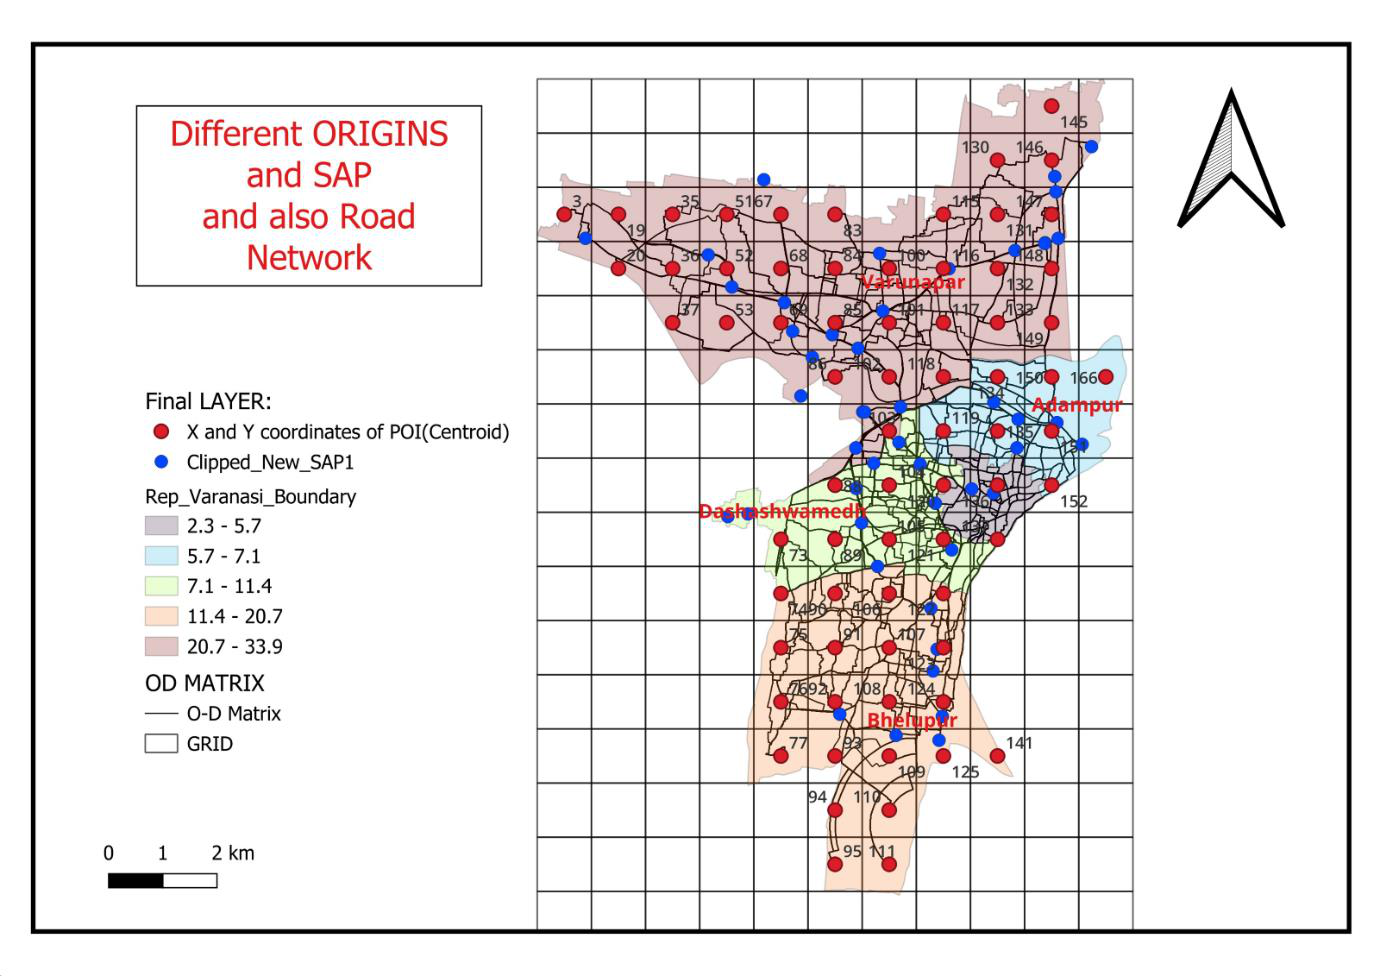
\includegraphics[width=0.85\textwidth]{fig_varanasi_poi_sap.png}
\caption{Points of interest (POI, red), service access points (SAP, blue), road network, and OD
matrix for Varanasi.}
\end{figure}

\begin{figure}[H]
\centering
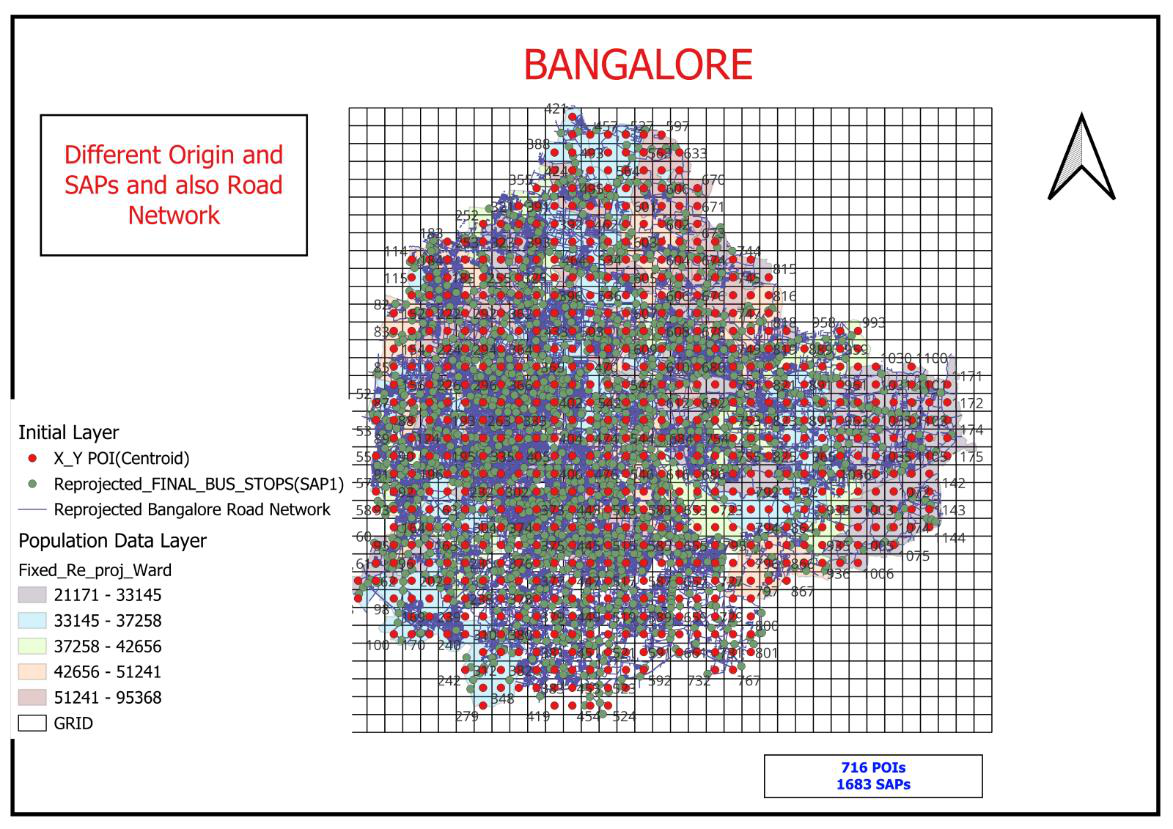
\includegraphics[width=0.85\textwidth]{fig_bangalore_poi_sap.png}
\caption{Points of interest (POI, red), service access points (SAP, green), road network, and
ward-wise population layer for Bangalore (716 POIs, 1683 SAPs).}
\end{figure}

\subsection{Applying the PTAL Method to the Bangalore and Varanasi Datasets}

\textbf{Step 1: Define points of interest (POI) and service access points (SAP).} A POI is a
point for which the accessibility level is to be measured with respect to an SAP, which is a
public transport stop (bus stop, metro station, etc.); in this study, bus stops serve as the
SAPs.

\textbf{Step 2: Calculate walk access time from POI to SAP.} The actual road-network distance
from POI to SAP is measured and, assuming the walk speeds in Table~\ref{tab:parameters}, the
walk time (WT) is calculated. SAPs beyond the maximum walk time are not considered when
estimating PTAL for that POI.

\textbf{Step 3: Identify valid routes at each SAP and calculate the average waiting time
(AWT).} Valid routes are bus and metro routes during the peak hour (8:00--10:00~AM), and the
frequency of services on all such routes during this hour is used in the AWT calculation:
\begin{equation}
\text{AWT} = 0.5\left(\frac{60}{f}\right) + K
\end{equation}
where AWT is the time between a passenger's arrival at an SAP and the arrival of the desired
service, the hourly frequency ($f$) is halved because the scheduled waiting time (SWT) is
estimated as half the headway, and a reliability factor ($K$) is added to the SWT depending on
the transport mode.

\textbf{Step 4: Calculate the minimum total access time (TAT) for each valid route at each
SAP.}
\begin{equation}
\text{TAT} = \text{WT} + \text{AWT}
\end{equation}

\textbf{Step 5: Convert TAT into equivalent doorstep frequency (EDF).} The principle is to
treat access time as a notional average waiting time as though the route were available at the
doorstep of the selected POI.
\begin{equation}
\text{EDF} = \frac{30}{\text{TAT}}
\end{equation}
The reason for dividing 30 (minutes) by TAT is that it re-applies the half-the-headway rule.
This is applied twice because the two values have different meanings. In Step~3, frequency is
converted into AWT; in Step~5, TAT is converted back into a frequency (EDF). TAT is a number
comparable to service frequency but takes into account the additional walk time to reach the
stop along with reliability; thus, the half-the-headway rule is applied again to TAT in Step~5 to
give the doorstep frequency.

\textbf{Step 6: Obtain the accessibility index (AI) for each POI.} The most dominant route
(the route with the highest frequency) is assigned a weighting factor of 1.0; for all other
routes, a weighting factor of 0.5 is assigned. For a transport mode ($m$):
\begin{equation}
(\text{AI})_m = (\text{EDF})_{\max} + 0.5 \sum_{\text{all other routes}} \text{EDF}
\end{equation}
and the accessibility index for a POI is
\begin{equation}
(\text{AI})_{\text{POI}} = \sum_m (\text{AI})_m
\end{equation}

\textbf{Step 7: Map PTAL.} The AIs obtained for each POI are allocated to eight PTAL bands as
in Table~\ref{tab:ptalbands} (for Bangalore) and Table~\ref{tab:varanasibands} (for Varanasi,
recalibrated for the smaller AI range observed there). A POI with a value of~0 indicates no
access to the public transport network within the given parameters and is left uncoloured on the
map.

\begin{table}[H]
\centering
\caption{PTAL score bands adopted for Varanasi.}
\label{tab:varanasibands}
\begin{tabular}{lll}
\toprule
\textbf{PTAL} & \textbf{Range of Index} & \textbf{Description} \\
\midrule
1a (Low) & 0.01--1.05 & Very Poor \\
1b       & 1.51--4.00 & Very Poor \\
2        & 4.51--7.00 & Poor \\
3        & 7.01--10.00 & Moderate \\
4        & 10.01--15.00 & Good \\
5        & 15.01--20.00 & Very Good \\
6a       & 20.01--30.00 & Excellent \\
6b (High) & $<$30 & Excellent \\
\bottomrule
\end{tabular}
\end{table}

\section{Results and Discussion}

\subsection{Comparison of PTAL Scores: Bangalore and Varanasi}

Figures~\ref{fig:banghmap} and \ref{fig:varmap} present the PTAL score maps for Bangalore and
Varanasi respectively, highlighting the areas with high, medium, and low accessibility.

\begin{figure}[H]
\centering
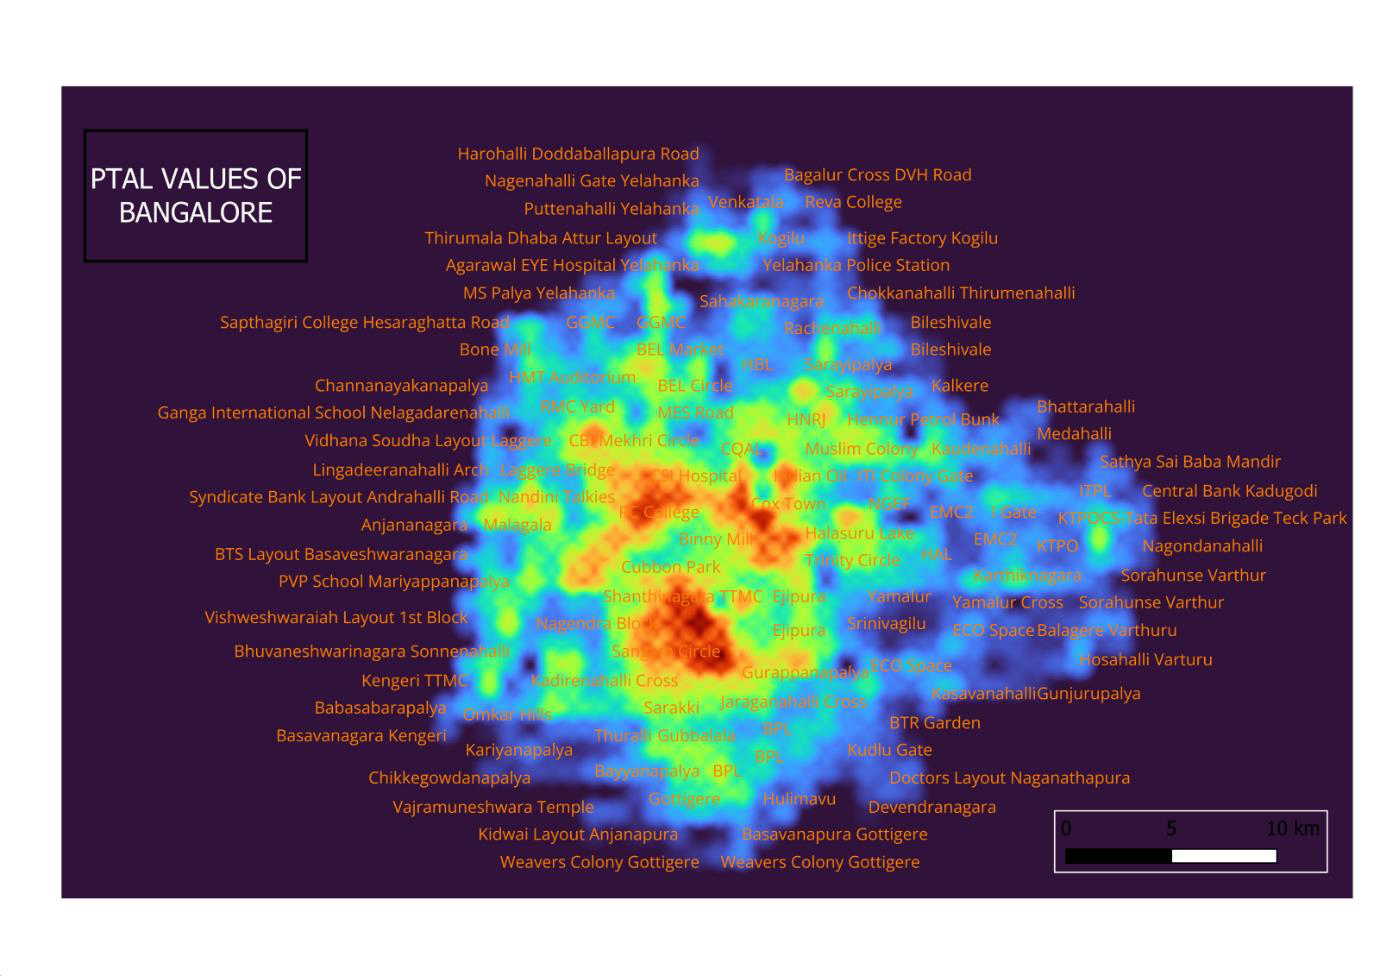
\includegraphics[width=0.85\textwidth]{fig_bangalore_ptal_heatmap.png}
\caption{PTAL heatmap of Bangalore, showing accessibility concentrated around the central
business district and declining toward the periphery.}
\label{fig:banghmap}
\end{figure}

\begin{figure}[H]
\centering
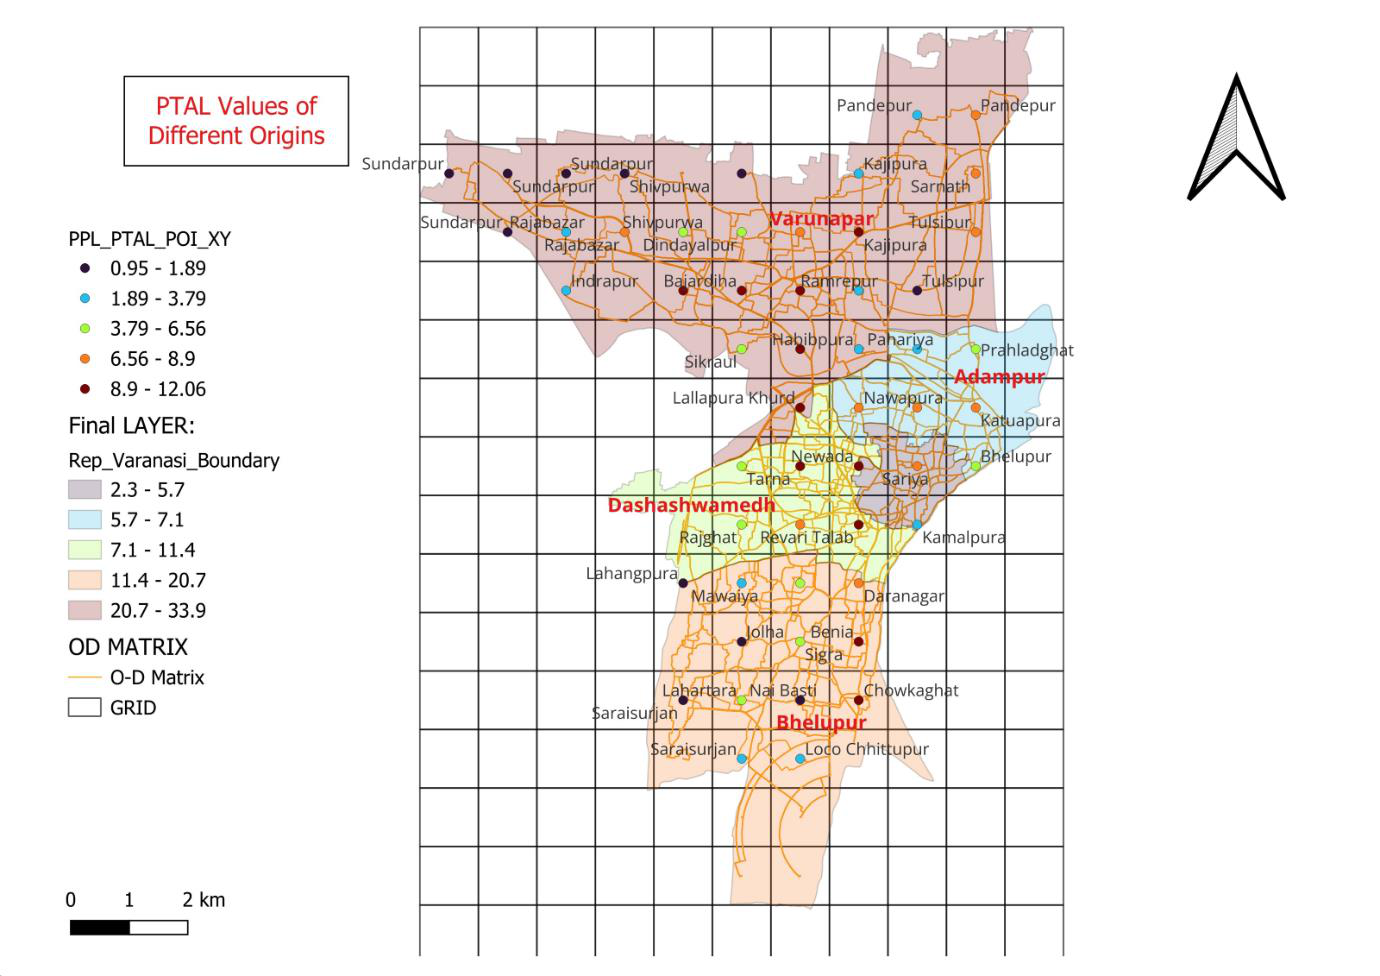
\includegraphics[width=0.7\textwidth]{fig_varanasi_ptal_map.png}
\caption{PTAL values across different origins in Varanasi, overlaid on ward boundaries
(Varunapar, Adampur, Dashashwamedh, Bhelupur, Kotwali).}
\label{fig:varmap}
\end{figure}

For Varanasi, the distribution of the 54 grid-cell scores across PTAL categories is shown in
Figure~\ref{fig:scoredist}: the majority of cells fall in the ``Moderate'' (PTAL~3, 33.3\%) and
``Very Poor'' (PTAL~1b, 27.8\%) bands, with smaller shares in ``Poor'' (14.8\%), ``Excellent''
(PTAL~6b, 9.3\%), ``Very Poor--Low'' (PTAL~1a, 9.3\%), and ``Good'' (PTAL~4, 5.6\%).

\begin{figure}[H]
\centering
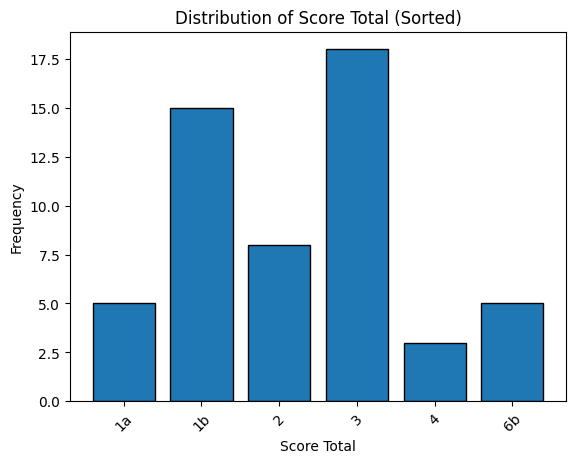
\includegraphics[width=0.75\textwidth]{fig_score_dist_bar.png}
\caption{Distribution of PTAL score-total categories across Varanasi grid cells.}
\end{figure}

\begin{figure}[H]
\centering
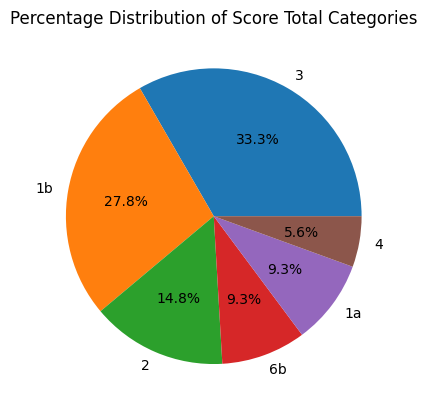
\includegraphics[width=0.55\textwidth]{fig_score_dist_pie.png}
\caption{Percentage distribution of PTAL score-total categories, Varanasi.}
\label{fig:scoredist}
\end{figure}

\subsection{Relationship Between PTAL Scores and Urban Characteristics}

To discuss the relationship between PTAL scores and population density, Varanasi's grid cells
were classified into six categories: Low PTAL with High Population, Moderate PTAL with High
Population, High PTAL with High Population, Low PTAL with Low Population, Moderate PTAL with
Low Population, and High PTAL with Low Population.

\textbf{Low PTAL with high population.} Several densely populated areas of Varanasi, namely
Shivpurwa, Pardepur, Tulsipur, Pahariya, Jolha, and Saraisurjan, combine high population with
poor accessibility (Figure~\ref{fig:lowhigh}). In Shivpurwa, limited road width and congestion
impede efficient bus manoeuvring, resulting in prolonged travel times, and the absence of
exclusive bus lanes compels buses to share road space with other vehicles, causing further
delays; overcrowded bus stops further inconvenience commuters. Pardepur's remote positioning on
the city outskirts complicates accessibility from the central district, with sparse bus services
hindering travel especially during non-peak hours, compounded by poor road conditions. Tulsipur
suffers from inadequate infrastructure (bus stops, signage, lighting) and uncoordinated bus
schedules that cause prolonged waits and missed connections. Pahariya's hilly topography and
narrow streets restrict bus navigation and limit route reach. Jolha experiences heavy peak-hour
congestion and inadequate parking that forces buses to stop inconveniently, disrupting flow. In
Saraisurjan, an insufficient bus fleet relative to the growing population results in
overcrowding and compromised accessibility, with inefficient routing potentially overlooking
population distribution and travel patterns.

\begin{figure}[H]
\centering
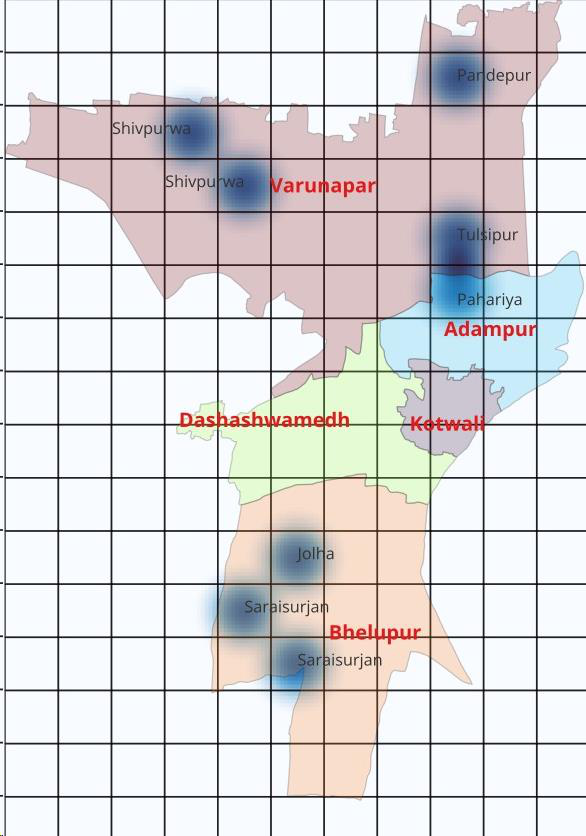
\includegraphics[width=0.55\textwidth]{fig_low_ptal_high_pop.png}
\caption{Low PTAL value with high population, Varanasi.}
\label{fig:lowhigh}
\end{figure}

\textbf{Moderate PTAL with high population.} Tarna and Nariya in Varanasi face escalating
demands for efficient public transport amid growing populations. While maintaining moderate
PTAL, a lack of proactive measures might lead to declining accessibility, posing risks including
amplified traffic congestion, diminished economic activity, environmental degradation, and
social disparities. The combined populace of this cluster surpasses 200,000, yielding a density
of over 30,000 individuals per square kilometre; the transport network comprises buses,
rickshaws, and auto-rickshaws, yet insufficient bus frequency and a lack of exclusive lanes
result in delays and congestion. Despite these challenges, over 60\% of residents rely on public
transport for commuting. Left unaddressed, growing populations could intensify congestion and
pollution, hinder economic access, and accelerate environmental deterioration; potential
solutions include expanding bus service coverage, designating dedicated bus lanes, enhancing
road network infrastructure, upgrading bus stop facilities, integrating public transport modes,
implementing real-time bus tracking, and employing data-driven decision-making.

\textbf{High PTAL with high population.} Nevada and Tulsipur, two densely populated
neighbourhoods, enjoy high PTAL owing to a combination of factors (Figure~\ref{fig:highhigh}):
strategic, centrally located positioning providing easy access to major employment hubs,
educational institutions, and commercial centres; an efficient, well-planned road network with
dedicated bus lanes enabling smooth traffic flow; adequately placed and frequent bus stops
ensuring easy access to public transport; and seamless integration with rickshaws and
auto-rickshaws allowing convenient onward travel.

\begin{figure}[H]
\centering
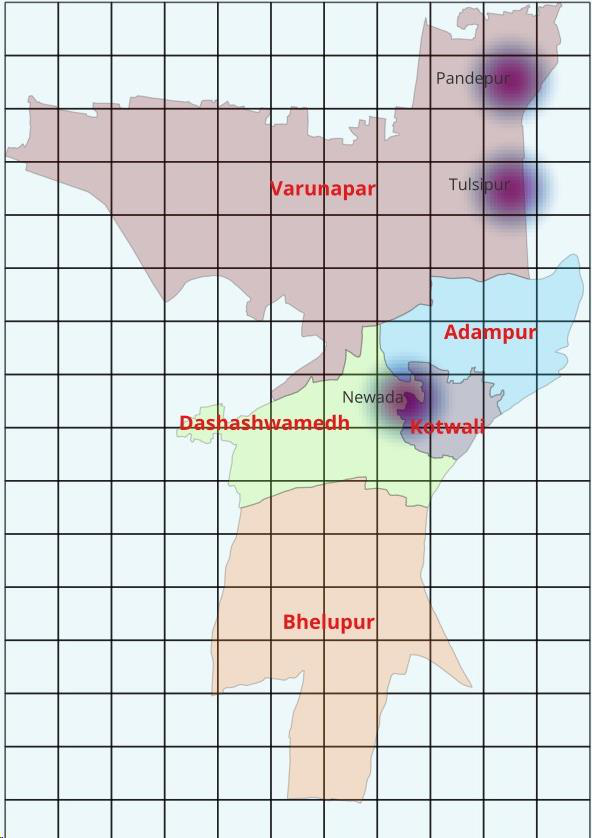
\includegraphics[width=0.55\textwidth]{fig_high_ptal_high_pop.png}
\caption{High PTAL with high population, Varanasi.}
\label{fig:highhigh}
\end{figure}

Corresponding lower-population variants of these categories were also examined (Low, Moderate,
and High PTAL with Low Population), confirming that population density alone does not determine
PTAL: several low-population grid cells still register poor accessibility due to peripheral
location or thin route coverage, while others enjoy high accessibility from proximity to
well-served corridors. Figure~\ref{fig:subplots} presents the full set of six PTAL-versus-population
subplots used to identify these categories.

\begin{figure}[H]
\centering
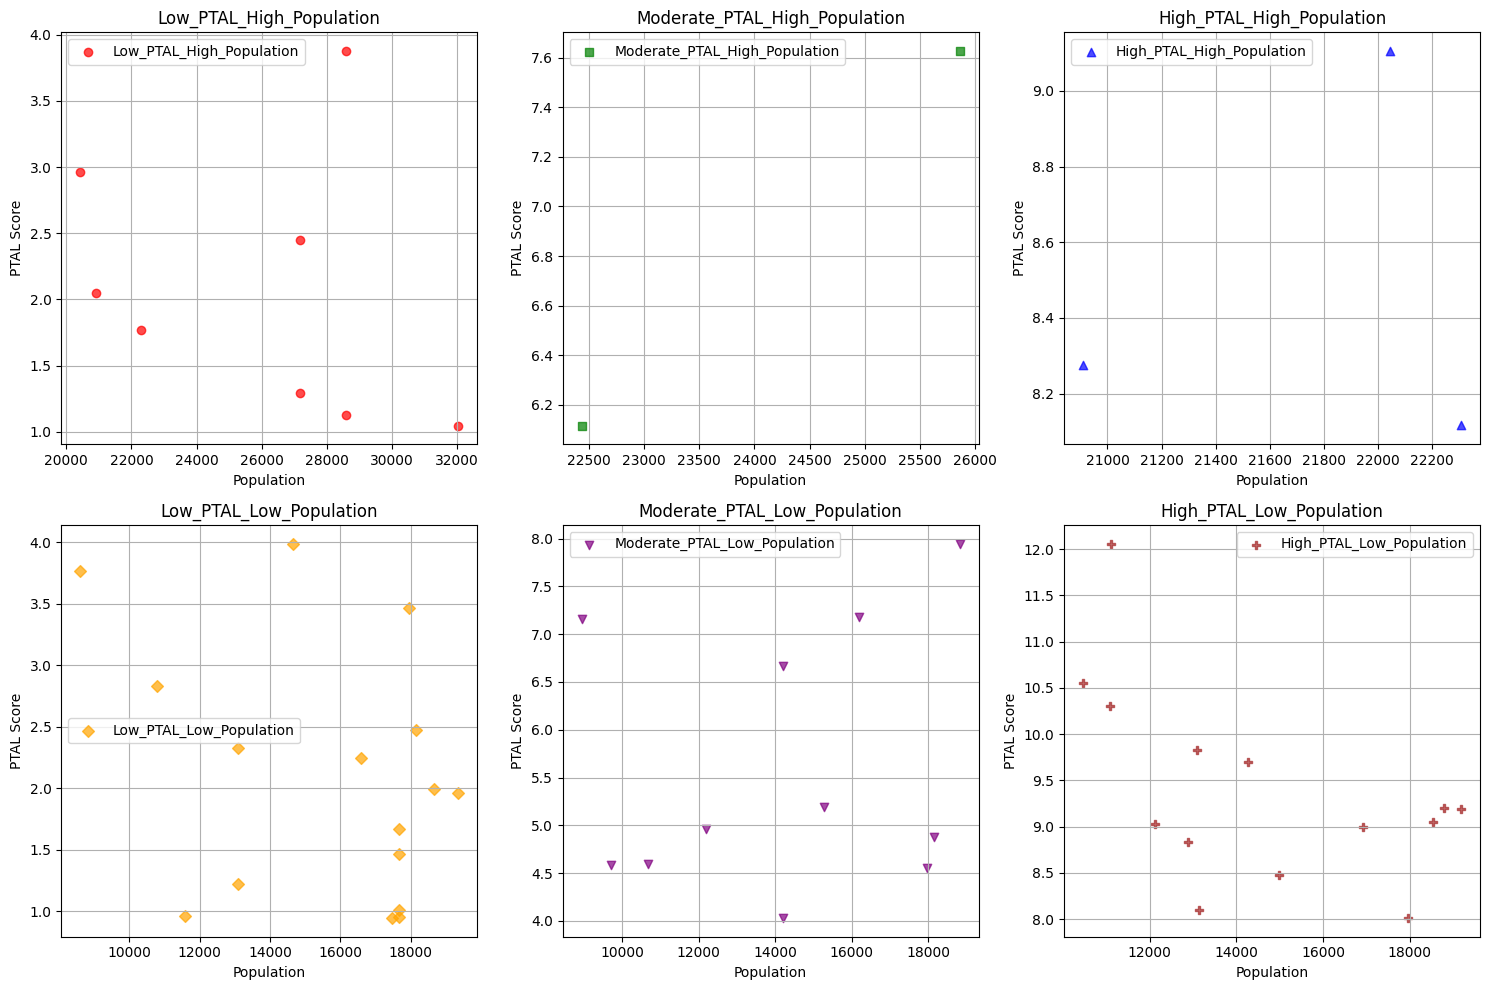
\includegraphics[width=0.95\textwidth]{fig_subplots_ptal_pop.png}
\caption{Subplots of PTAL score against population across the six identified categories,
Varanasi.}
\label{fig:subplots}
\end{figure}

\subsection{Regression Analysis: Comparison Between Varanasi and Bangalore}

In the comparison of Regression Analysis between the Varanasi and Bangalore datasets, several
vital distinctions and similarities emerge, shedding light on their respective public transport
accessibility landscapes.

\subsubsection{For Varanasi}

Figure~\ref{fig:varbubble} shows the bubble plot of PTAL score against population for the six
identified categories, and Figure~\ref{fig:varreg} shows the fitted OLS regression line.

\begin{figure}[H]
\centering
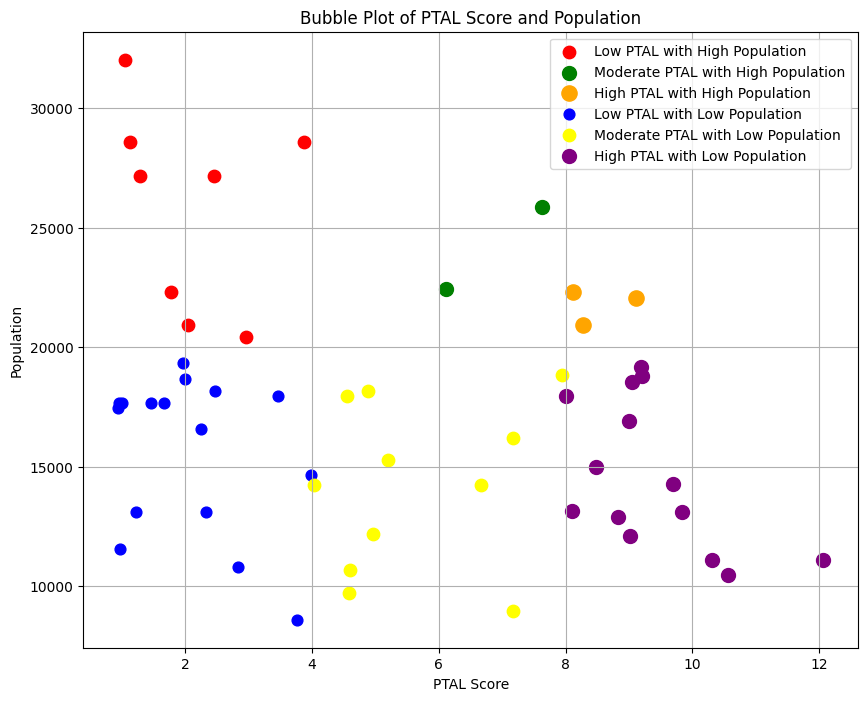
\includegraphics[width=0.75\textwidth]{fig_varanasi_bubble.png}
\caption{Bubble plot of PTAL score and population, Varanasi.}
\label{fig:varbubble}
\end{figure}

\begin{figure}[H]
\centering
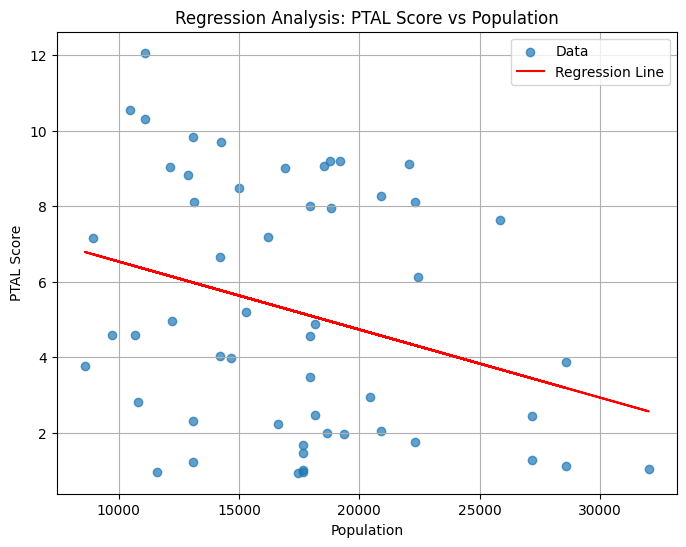
\includegraphics[width=0.7\textwidth]{fig_varanasi_regression.png}
\caption{Regression analysis of PTAL score vs.\ population, Varanasi.}
\label{fig:varreg}
\end{figure}

The regression analysis conducted between population and PTAL score for Varanasi yields the
following insights:
\begin{itemize}
  \item \textbf{R-squared and adjusted R-squared:} an R\textsuperscript{2} of 0.086 suggests
  that changes in population can explain approximately 8.6\% of the variability in PTAL scores;
  the adjusted R\textsuperscript{2}, accounting for the number of predictors, stands at 0.068.
  \item \textbf{Significance of the population coefficient:} the coefficient for population is
  $-0.0002$ with a p-value of 0.031, suggesting that for every unit increase in population, the
  PTAL score decreases by 0.0002; the coefficient's p-value is below 0.05, indicating some
  significance, though the effect size is notably small.
  \item \textbf{Intercept coefficient:} the intercept value is 8.3325, indicating an estimated
  PTAL score of approximately 8.33 when the population is zero.
  \item \textbf{Model significance:} an F-statistic of 4.888 with p-value 0.0315 suggests the
  overall regression model is statistically significant at the 0.05 level.
  \item \textbf{Model fit:} the low R-squared value indicates that the model does not fully
  capture the variability in PTAL scores, and other factors likely play a more substantial role.
\end{itemize}

The analysis shows a statistically significant, albeit weak, \emph{negative} relationship
between population and PTAL score in Varanasi: an increase in population might marginally lead
to a slight decrease in PTAL scores. This finding suggests that Varanasi's growing population may
pose a challenge in maintaining and improving public transport accessibility, potentially due to
overburdened infrastructure (bus routes, stops, and fleet size becoming strained as population
grows, leading to overcrowding and reduced accessibility), traffic congestion (increased
population density making it more difficult for buses to navigate efficiently), and limited
resources (constrained ability to expand the network to meet growing demand).

A declining PTAL trend could also affect Varanasi's cultural heritage: reduced accessibility to
cultural sites (temples, ghats, museums) could hinder tourists and residents from fully
experiencing the city's offerings; limited mobility could restrict participation in cultural
events and gatherings, particularly for older residents and those with disabilities; and
increased pressure on public transport could strain cultural infrastructure such as bus stops and
terminals near heritage sites. Possible solutions include expanding the public transport network
(new routes, more bus stops, upgraded infrastructure), implementing traffic management measures
(dedicated bus lanes, signal optimisation, congestion pricing), optimising resource allocation
(public--private partnerships, technology for service optimisation), integrating cultural
sensitivity into transport planning so that heritage sites remain well-connected, and engaging
local communities and cultural institutions in transport development plans.

\subsubsection{For Bangalore}

Figure~\ref{fig:bangbubble} shows the bubble plot of PTAL score and 2022 population estimate for
Bangalore, and Figure~\ref{fig:bangreg} shows the fitted regression line.

\begin{figure}[H]
\centering
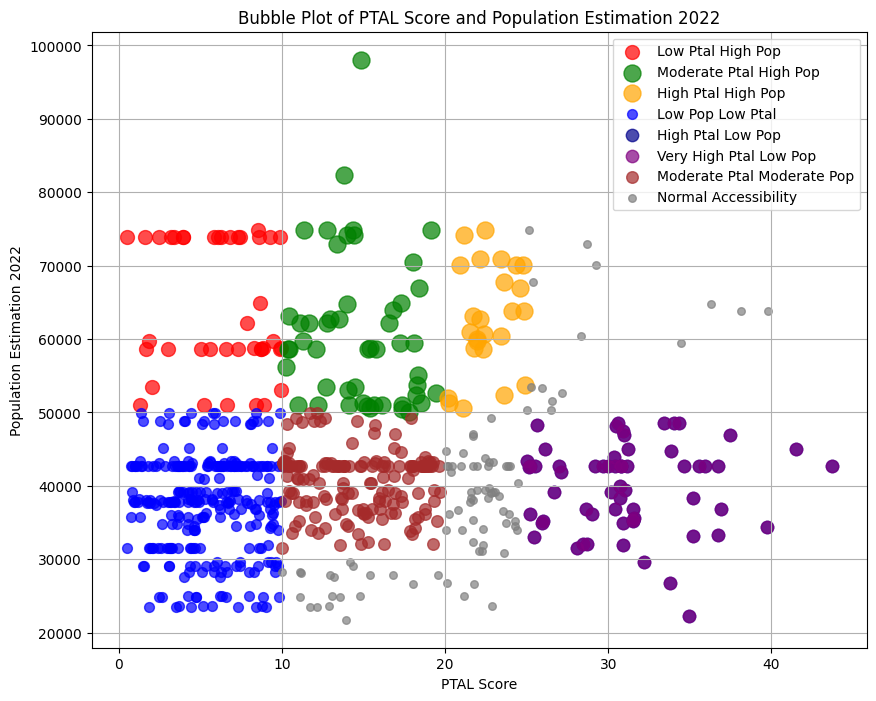
\includegraphics[width=0.75\textwidth]{fig_bangalore_bubble.png}
\caption{Bubble plot of PTAL score and 2022 population estimate, Bangalore.}
\label{fig:bangbubble}
\end{figure}

\begin{figure}[H]
\centering
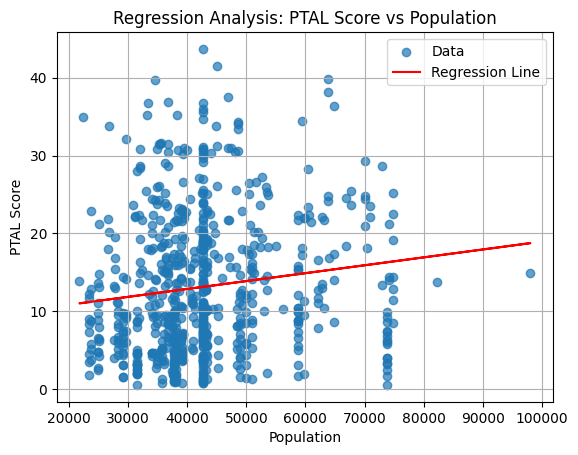
\includegraphics[width=0.7\textwidth]{fig_bangalore_regression.png}
\caption{Regression analysis of PTAL score vs.\ population, Bangalore.}
\label{fig:bangreg}
\end{figure}

The regression analysis between population estimation and PTAL score in Bangalore revealed a
statistically significant but weak \emph{positive} relationship, suggesting that an increase in
population tends to lead to a slight rise in PTAL score. This finding indicates that Bangalore's
growing population could potentially benefit from improved public transport accessibility,
attributable to infrastructure development (a corresponding expansion of public transport
infrastructure, such as new bus routes, metro lines, and bus rapid transit corridors, leading to a
more extensive and accessible network), policy initiatives (subsidies for bus fares, dedicated bus
lanes, and integrated ticketing systems encouraging more residents to switch to public
transport), and technological advancements (real-time bus tracking apps, mobile ticketing, and
intelligent traffic management systems improving travel planning and reducing waiting times).

Improved PTAL in Bangalore has several implications for the business environment: enhanced
employee mobility through a well-connected public transport system reducing commute time;
reduced traffic congestion easing the movement of goods and services; access to a wider talent
pool as improved accessibility allows businesses to draw from a larger and more diverse
workforce; and support for sustainable urban development by reducing reliance on private
vehicles. Possible strategies to further enhance PTAL in Bangalore include continued
infrastructure expansion (prioritising high-demand business hubs and under-connected residential
areas), integration with other modes (autos, rickshaws, bicycles for first- and last-mile
connectivity), demand-responsive transport in areas of low density or fluctuating demand,
data-driven decision-making to identify low-accessibility areas, and public--private
partnerships.

\subsection{Comparison of Regression Results}

Table~\ref{tab:comparison} summarises the regression results for the two cities.

\begin{table}[H]
\centering
\caption{Comparison of regression results: Varanasi vs.\ Bangalore.}
\label{tab:comparison}
\begin{tabular}{lcc}
\toprule
\textbf{Feature} & \textbf{Varanasi} & \textbf{Bangalore} \\
\midrule
R-squared & 0.086 & 0.018 \\
Population coefficient & $-0.0002$ (p = 0.031) & $0.0001$ (p = 0.000441) \\
Intercept & 8.3325 & 8.7965 \\
F-statistic and p-value & 4.888 (p = 0.0315) & 12.47 (p = 0.000441) \\
\bottomrule
\end{tabular}
\end{table}

\textbf{Key insights.} The direction of the relationship between population and PTAL score
differs between the two cities: Varanasi has a weak negative relationship, suggesting that
increasing population tends to lead to a slight decrease in PTAL score, whereas Bangalore
exhibits a weak positive relationship, indicating that population growth is associated with a
slight increase in PTAL score. The strength of the relationship also differs: in Varanasi, the
R-squared value of 0.086 suggests that only about 8.6\% of the variability in PTAL scores can be
explained by population, whereas in Bangalore the R-squared value of 0.018 is even lower,
indicating population alone explains only about 1.8\% of the variability. The significance of the
population coefficient also differs: in Varanasi, the p-value of 0.031 suggests the negative
relationship is statistically significant at the 5\% level, while in Bangalore the p-value of
0.000441 indicates even more robust statistical significance for the positive relationship.

\textbf{Possible explanations for the differences.} Bangalore has invested more heavily in
public transport infrastructure, such as metro lines, bus rapid transit corridors, and dedicated
bus lanes, compared to Varanasi, likely contributing to the positive population--PTAL relationship
observed there. Bangalore has also implemented various policies to promote public transport
usage, including subsidies, integrated ticketing systems, and priority lanes, further improving
accessibility as the population grows. Bangalore's urban planning and transportation master
plans have emphasised the development of a comprehensive and interconnected public transport
network, while Varanasi's urban planning may not have prioritised public transport to the same
extent. Finally, Bangalore's economic growth and vibrant business environment have driven
investment in infrastructure and policy initiatives supporting accessibility.

\section{Conclusion}

The comparative analysis of PTAL scores in Bangalore and Varanasi highlights the importance of
considering factors beyond population growth alone when assessing and improving public transport
accessibility. Cities like Varanasi can learn from Bangalore's experience by prioritising public
transport infrastructure, implementing supportive policies, and adopting comprehensive urban
planning strategies that promote a well-connected and accessible public transport system. By
addressing their unique challenges and leveraging their respective strengths, both Varanasi and
Bangalore can continue to enhance their PTAL scores, ensuring sustainable mobility, improved
quality of life for residents, and a more attractive environment for businesses to thrive.

The grid-based PTAL mapping approach developed in this study, adapted from the London/TfL
methodology to the data constraints and urban form of Indian cities, offers a quantitative,
transferable measure of accessibility to public transport that can inform planning practice in
several ways: formulating development/master plans with land use--transport integration,
prioritising public transport and supporting investment in low-accessibility areas, formulating
parking policies that discourage private vehicle use where PTAL is already high, and developing
transit-oriented zoning regulations that concentrate density around high-PTAL nodes.

\begin{thebibliography}{99}

\bibitem{handy2002}
Handy, S.\ (2002). Accessibility- vs.\ mobility-enhancing strategies for addressing automobile
dependence in the U.S. \textit{European Conference of Ministers of Transport}.

\bibitem{banister2006}
Banister, D., \& Hickman, R.\ (2006). How to design a more sustainable and fairer built
environment: transport and communications. \textit{IEE Proceedings -- Intelligent Transport
Systems}, 153(4), 276--291.

\bibitem{cervero1997}
Cervero, R., \& Kockelman, K.\ (1997). Travel demand and the 3Ds: density, diversity, and
design. \textit{Transportation Research Part D: Transport and Environment}, 2(3), 199--219.

\bibitem{guo2015}
Guo, Z., \& Wilson, N.\ H.\ M.\ (2015). Transit service and equity: a review. \textit{Journal of
Transport Geography}, 44, 15--25.

\bibitem{adhvaryu2010}
Adhvaryu, B.\ (2010). Land use and transport integration modeling for Ahmedabad. In
\textit{12th World Conference on Transport Research (WCTR)}, Lisbon, Portugal.

\bibitem{adhvaryu2011}
Adhvaryu, B.\ (2011). Sustainable transport planning in India: a critical review. \textit{Journal
of Public Transportation}, 14(2), 1--26.

\bibitem{adhvaryu2017}
Adhvaryu, B., \& Kumar, P.\ (2017). Accessibility planning and modeling: a review of practices
and challenges. \textit{Journal of Transport Geography}, 64, 116--130.

\bibitem{adhvaryu2015}
Adhvaryu, B.\ (2015). Evaluation of land use transport integration in Indian cities: an
empirical study of Ahmedabad. \textit{Journal of Transport and Land Use}, 9(1), 1--23.

\bibitem{adhvaryu2014}
Adhvaryu, B.\ (2014). Assessing the impact of a Bus Rapid Transit (BRT) system on accessibility
and social equity: a case study of Ahmedabad, India. \textit{Journal of Transport Geography}, 41,
180--191.

\bibitem{adhvaryu2013}
Adhvaryu, B., \& Kanth, S.\ A.\ (2013). Evaluation of public transport system using
AHP -- a case study of Ahmedabad city. \textit{Transportation Research Part A: Policy and
Practice}, 49, 247--257.

\bibitem{adhvaryu2012}
Adhvaryu, B., \& Kanth, S.\ A.\ (2012). Modeling public transport network accessibility in
Ahmedabad, India. \textit{Journal of Transport Geography}, 22, 244--251.

\bibitem{das2014}
Das, S., \& Sivakumar, A.\ (2014). A study on public transport system in Bangalore city.
\textit{International Journal of Innovative Research in Science, Engineering, and Technology},
3(10), 16692--16699.

\bibitem{mohua2019}
Ministry of Housing and Urban Affairs (2019). \textit{Smart Cities Mission: Comprehensive
Mobility Plan}. Government of India.

\bibitem{niua2014}
National Institute of Urban Affairs (2014). \textit{Sustainable Urban Transport Project:
Bangalore City Diagnosis}. Ministry of Urban Development, Government of India.

\bibitem{planningcomm2011}
Planning Commission of India (2011). \textit{Report of the Working Group on Urban Transport for
the Twelfth Five Year Plan (2012--17)}. Government of India.

\bibitem{trb2013}
Transportation Research Board (2013). \textit{Transit Capacity and Quality of Service Manual}
(3rd ed.). Transit Cooperative Research Program, National Research Council.

\end{thebibliography}

\end{document}
